% Chapter Template

\chapter{Experimental Evaluation} % Main chapter title

\label{Chapter5} % Change X to a consecutive number; for referencing this chapter elsewhere, use \ref{ChapterX}

\lhead{Chapter 5. \emph{Experimental Evaluation}} % Change X to a consecutive number; this is for the header on each page - perhaps a shortened title

This chapter's purpose is to verify the correctness and the efficiency of SparkSQL Server. Due to the limitation of time, in its current state the experiment is designed to be simple. We design the experiments on sharing scan with an input file of 10GB and various Window size of the DAG Queue at SparkSQL Server on two techniques: caching of Spark and sharing map input of MRShare.\\
From these experiments, we evaluate the performance of caching technique and also verify the performance of sharing map input of MRShare, which originally works on Apache Hadoop Mapreduce, on Apache Spark.


%-----------------------------------
%	SUBSECTION 1
%-----------------------------------
\section{Experimental Setup}
Our experimental evaluation is done on a YARN cluster with 17 nodes, each has 4 vcores and 6GB of RAM. Our Apache Spark is modified from version 1.3.1. All results shown in the following are the average of 5 runs: the standard deviation is smaller than 2.5 "\%", hence – for the sake of readability – we omit error bars from our figures.\\
The input files we use are taken from Project Gutenberg, which provides a collection of full texts of public domain books. The size of the input file is 10GB. We take the common used WordCount program for both caching experiment and grep-WordCount for MRShare technique experiment since the paper on MRShare also used grep-WordCount to evaluate their works. In our experiment, with the grep-WordCount, we filter the length of each word to control the map output size of each job. We choose the Window Size of the Queue at SparkSQL Server with 2 then 5 and 10.\\
We compare the total runtime of batch of jobs after going through SparkSQL Server and that batch of jobs which is executed one by one without using scan sharing optimization.

%-----------------------------------
%	SUBSECTION 2
%-----------------------------------

\section{Results and Evaluations}
\begin{figure}
\includegraphics[width=\textwidth]{Figures/caching-vs-non-caching.eps}
\caption{Performance comparison with jobs submitted by SparkSQL Server and by users, using Caching}
\label{fig:caching}
\end{figure}

\begin{figure}
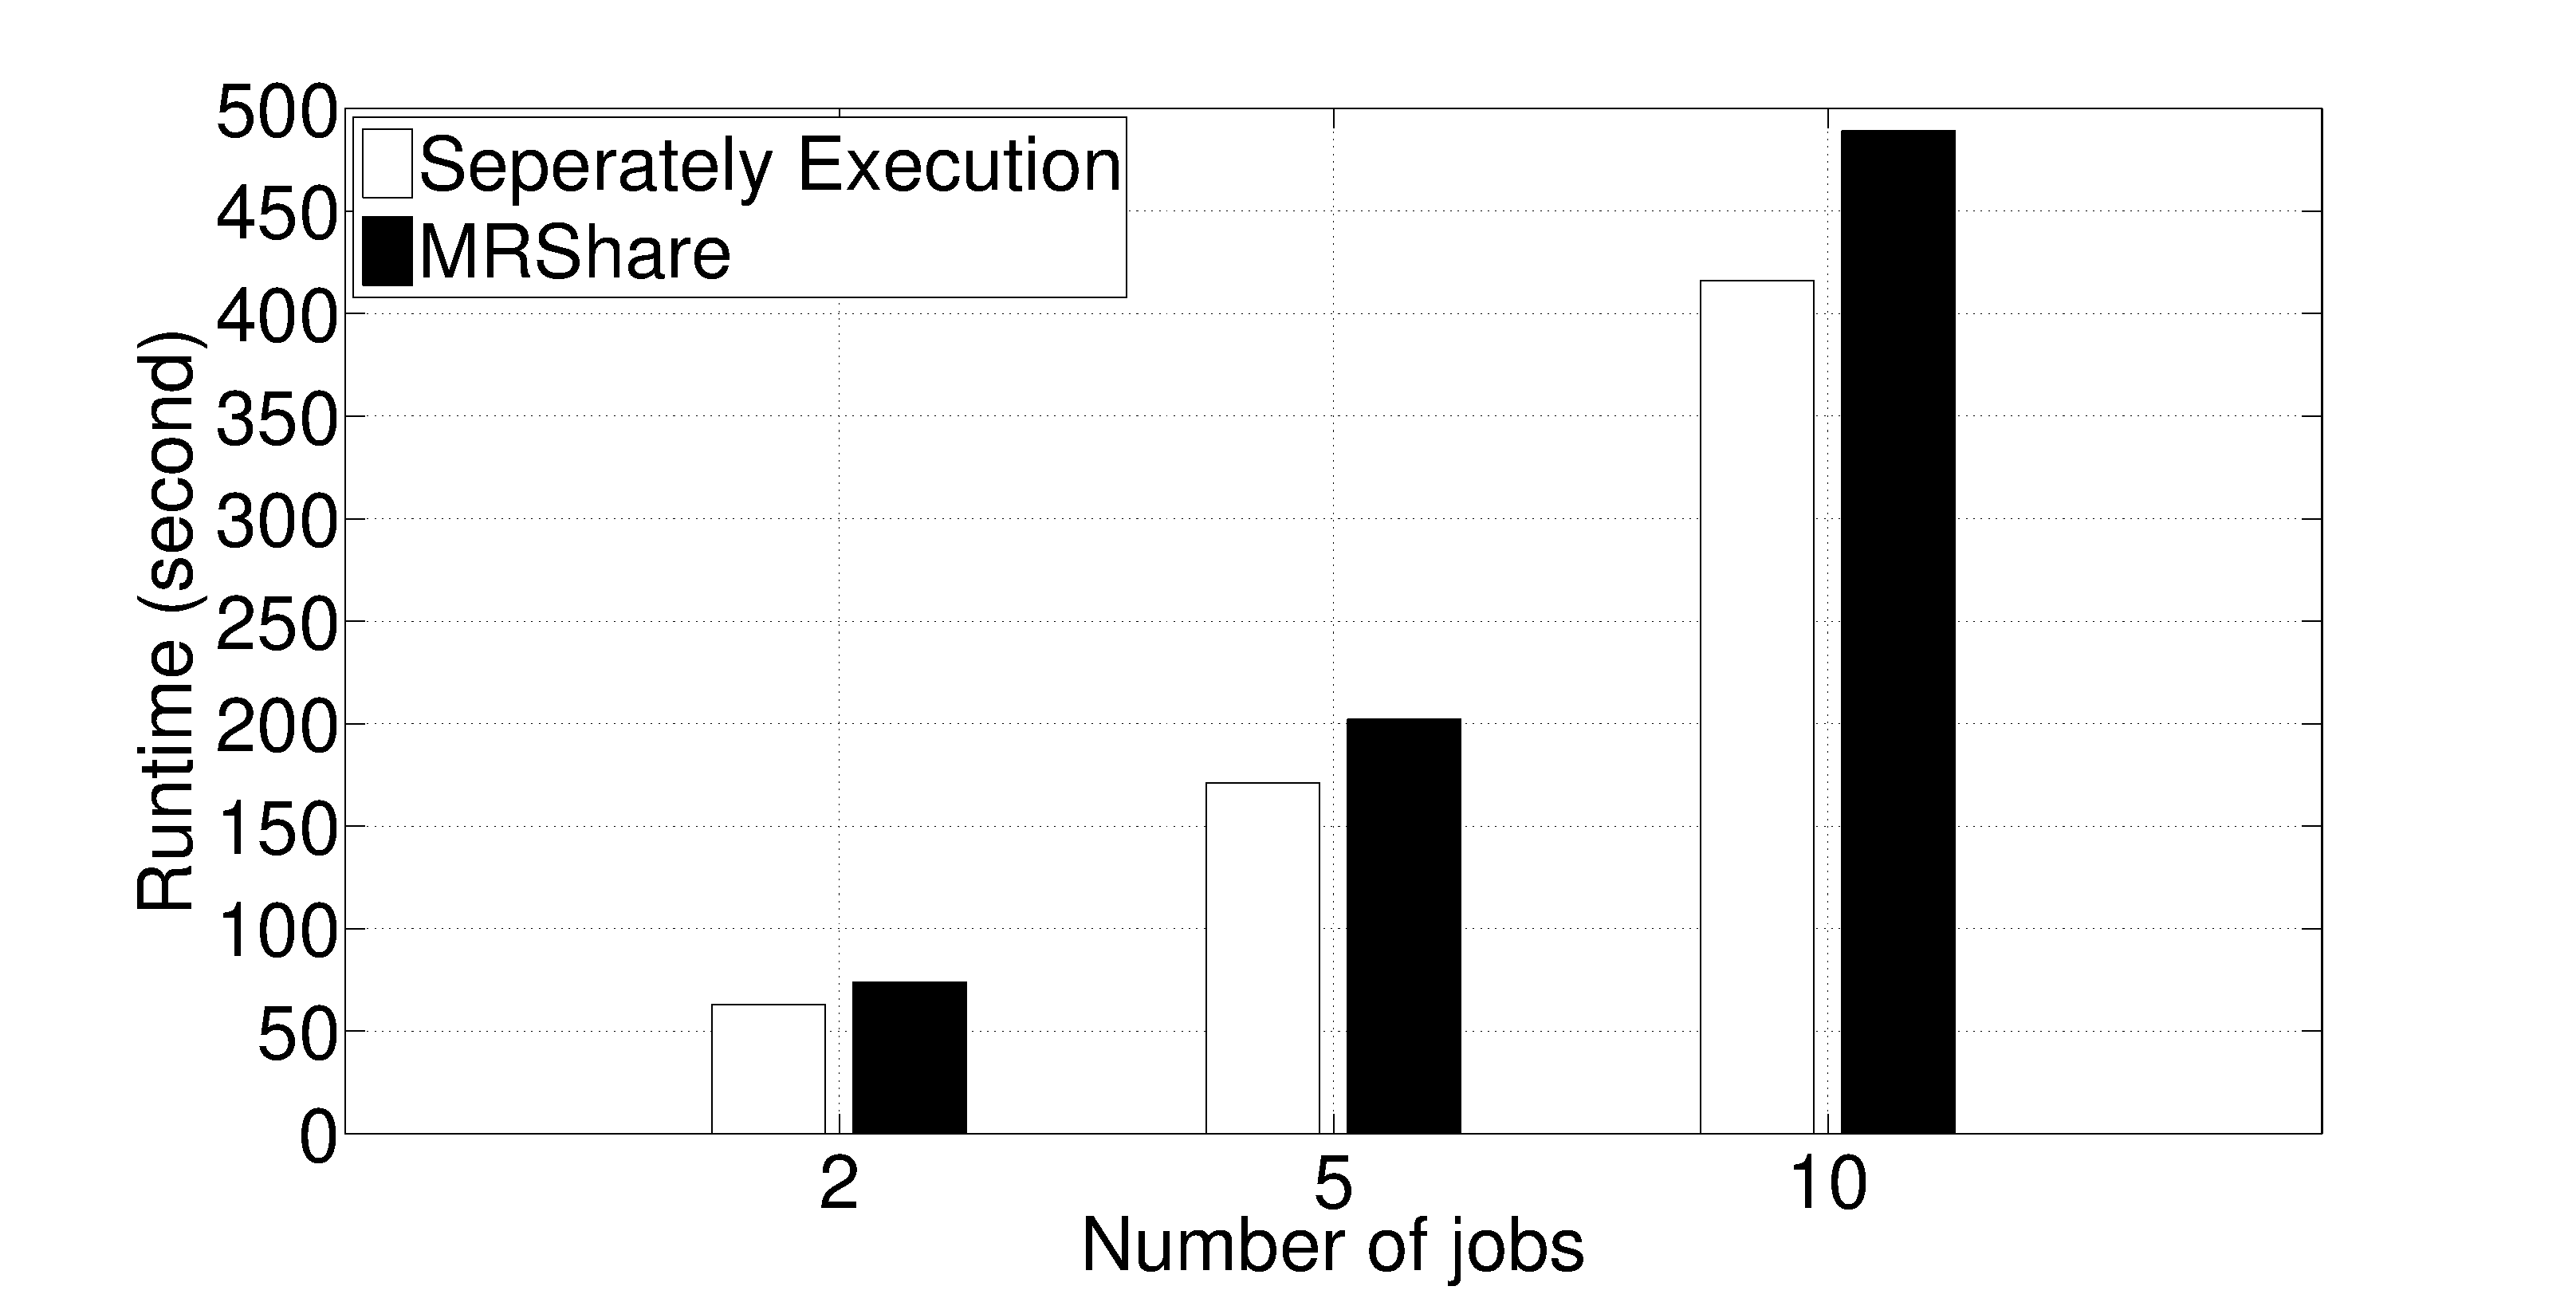
\includegraphics[width=\textwidth]{Figures/multi-mrshare.eps}
\caption{Performance comparison with job submitted by SparkSQL Server and by users, using MRShare}
\label{fig:mrshare}
\end{figure}

\begin{figure}
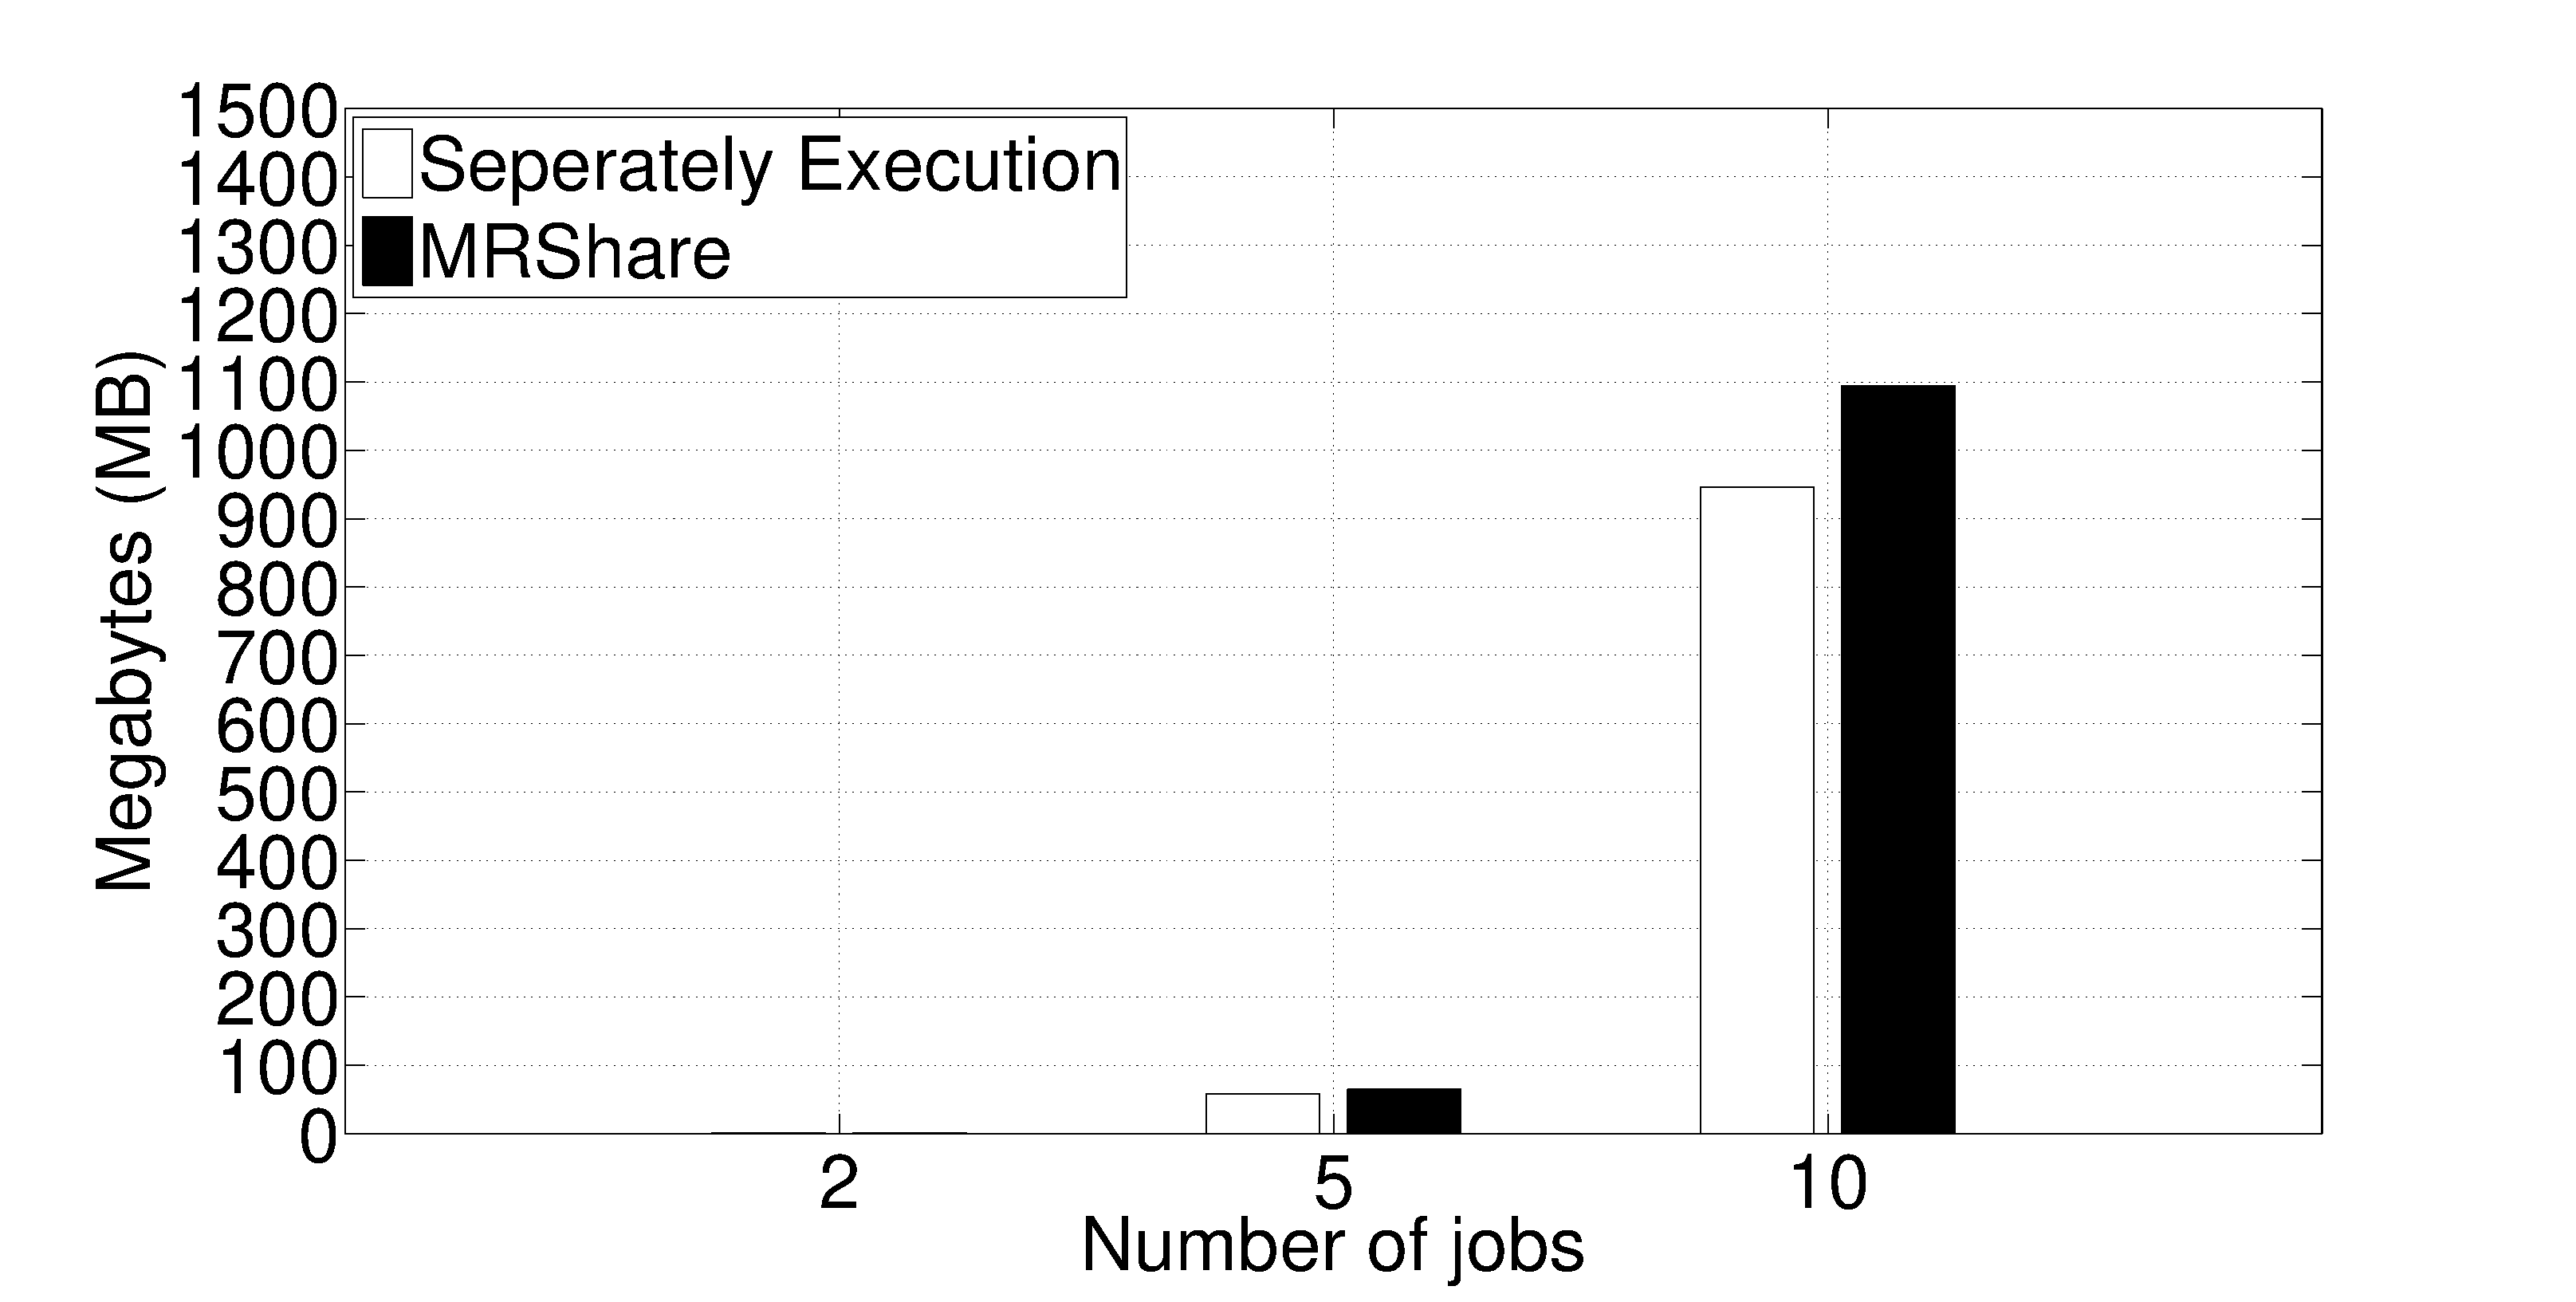
\includegraphics[width=\textwidth]{Figures/shuffle.eps}
\caption{Shuffle bytes of seperately execution and MRShare}
\label{fig:shuffle}
\end{figure}

With caching technique, as illustrated in figure \ref{fig:caching} for number of jobs varies from 2 to 10, batch of jobs going through SparkSQL Server has total runtime smaller than those jobs which are executed seperately. The saving using caching is not large in comparison to the total amount of time. This means that the sharing scan benefits do not dominant the sharing of computations. The SparkSQL Server functions well and gives the better performance rather than running those jobs submitted by users seperately.\\

Figure \ref{fig:mrshare} describes the performance of jobs submitted by SparkSQL Server and by users, using MRShare sharing technique. With sharing map input technique of MRShare. The total runtime of batch of jobs submitted by SparkSQL Server is larger than the total runtimes of those jobs submitted separately by users. The larger number of jobs are merged into a group, the larger total runtime it is. There are two reasons to explain this result and they are not related to the SparkSQL Server:\\
\begin{itemize}
\item In Apache Spark, a tuple  is immutable. So, when we do the tagging, we can not modify directly on the original tuple but need to generate a new tuple. We create too many objects and the Garbage Collector needs to take more time to do it job. MRShare produces 1 meta jobs for 2 jobs submitted, 2 meta jobs which are created by merging 2 and 3 seperated jobs, and 3 meta jobs which are created by merging 3, 3 and 4 seperated jobs. We sum the average of garbage collector runtime of those meta jobs and also sum the average of garbage collector runtime of seperated jobs. Table \ref{gc-runtime} shows the average of Garbage Collector runtime between MRShare technique and executing jobs separately. The more jobs are merged into a single meta job, the larger the average of garbage collector runtime is. In Apache Hadoop MapRedue, the record is mutable so it can reduce the cost of Garbage Collector.
\item The tagging operation is also a costly operation since larger data is shuffled over the network. Figure \ref{fig:shuffle} illustrates the different of shuffle bytes over the network of seperately job execution and MRShare technique. Each tuple also carries a label inside it so the shuffle bytes of MRShare technique is always larger. For 2 jobs, the shuffle bytes difference between two techniques is not so much, but for 5 jobs and 10 jobs, the shuffle bytes difference can affect the performance.
\end{itemize}

We make a simple experiment by creating a Spark application that we manually replicate the input tuple and tag the labeling into it. The number of replications is also varied from 2 then 5 and 10. The total runtime of MRShare technique is equal or smaller than the total runtime of executing jobs seperately, which means that the tagging technique is a costly operation. The original works of MRShare does not include the tagging cost into their cost model although through experiments, we realize that the cost of tagging is not negligible.

\begin{table}[]
\centering
\caption{Garbage Collector Average Runtime}
\label{gc-runtime}
\begin{tabular}{|l|l|l|}
\hline
Number of jobs & Seperately executed & MRShare \\ \hline
2              & 20 ms                  & 35 ms    \\ \hline
5              & 85 ms                  & 235 ms    \\ \hline
10             & 622 ms                 & 1369 ms   \\ \hline
\end{tabular}
\end{table}

The result of MRShare technique shows that the MRShare does not work as well as it does on Hadoop MapReduce since it is originally designed for MapReduce. In other words, the simultaneous pipeline technique that MRShare for Hadoop MapReduce uses is not suitable on Apache Spark due to the nature of each framework.\\

For caching approach, the results we obtain are not attractive since we just reduce the total execution time from 2 \% to 10 \%. For MRShare approach, the results are even worser due to the reasons we explain above. There is another reason which can explain our result: as a study on performance in data analytics frameworks \cite{kay2015} shows that for many simple jobs on Apache Spark, they are often bottlenecked on CPU and not I/O. That would explain more about the results we obtain. In addition, due to the limitation of time, we did not experiment enough on many kinds of workloads. We let this as a part of our future works.

From both experiments, the SparkSQL Sever proves its correctness. It also shows the extensibility of the system since we can easily add new sharing technique into the system.